\synctex=1
\documentclass[12pt,a4paper,oneside]{article}

\usepackage[spanish]{babel}

\usepackage{fancyhdr}
\usepackage{geometry}
\usepackage{graphicx}
\usepackage{wrapfig}
\usepackage{lastpage}
\usepackage[hidelinks]{hyperref}
\usepackage{authblk}
\usepackage{bookmark}

\usepackage[utf8]{inputenc} % Required for inputting international characters
\usepackage[T1]{fontenc} % Output font encoding for international characters
\usepackage{mathpazo} % Palatino font

\makeatletter
\newcommand{\subtitledoc}[1]{\newcommand{\@subtitledoc}{#1}}
\newcommand{\instituto}[1]{\newcommand{\@instituto}{#1}}
\newcommand{\carrera}[1]{\newcommand{\@carrera}{#1}}
\newcommand{\professor}[1]{\newcommand{\@professor}{#1}}
\newcommand{\catedraCaratula}[1]{\newcommand{\@catedraCaratula}{#1}}
\newcommand{\catedraHeader}[1]{\newcommand{\@catedraHeader}{#1}}
\newcommand{\curso}[1]{\newcommand{\@curso}{#1}}
\newcommand{\legajo}[1]{\newcommand{\@legajo}{#1}}
\newcommand{\footerauthor}[1]{\newcommand{\@footerauthor}{#1}}
\newcommand{\footerlegajo}[1]{\newcommand{\@footerlegajo}{#1}}

%Configuracion de hoja (margenes y tamaño)
\geometry{a4paper,margin=1in}
\setlength\headheight{28pt}

%formato de encabezado y pie para todas las paginas.
\fancyhead[L]{
    \begin{minipage}[b]{7.5mm}
        
\includegraphics[width=7mm]{Imagenes/logo-utn.png}
    \end{minipage}
    \begin{minipage}[b]{90mm}
        \textbf{Alumnos: }\@footerauthor \\
        \textbf{Legajos: }\@footerlegajo
    \end{minipage}
}
\fancyhead[R]{
    \textbf{Curso:} \@curso\\
    \textbf{Cátedra:} \@catedraHeader
}
\fancyfoot[L]{\@date}
\fancyfoot[C]{} %eliminar antiguo numero de pagina
\fancyfoot[R]{Página \thepage\ de \pageref{LastPage}}
\renewcommand{\headrulewidth}{0.5pt}
\renewcommand{\footrulewidth}{0.5pt}
\pagestyle{fancy}

\addto\captionsspanish{%
	\renewcommand{\contentsname}%
	{CONTENIDO}%
}

\renewcommand{\maketitle}{%
    \newpage
    \thispagestyle{empty}
    
    \begin{center}

    \textsc{\LARGE \@instituto}\\[0.5cm] 
    \textsc{\Large \@carrera}\\[1.5cm] 
    
\includegraphics[width=0.30\textwidth]{Imagenes/logo-utn.png} \par
    \vspace{1.5cm}
    
    \textsc{\large \@catedraCaratula }\\[0.5cm]
    
    {\huge\bfseries \@title}\\[0.4cm]
    \textsc{\Large \@subtitledoc}\\[0.5cm]
    

    \end{center}

    \vspace{2cm}

    {\noindent
    \begin{minipage}[t]{.2\textwidth}
        \raggedright
        \textbf{ALUMNOS} \par
        ~\\
        ~\\
        ~\\
        \textbf{CURSO} \par
        ~\\
        \textbf{DOCENTES} \par
        \end{minipage}%
     \begin{minipage}[t]{.05\textwidth}
        \raggedright
        \textbf{:} \par
        ~\\
        ~\\
        ~\\
        \textbf{:} \par
        ~\\
        \textbf{:} \par
    \end{minipage}%
    \begin{minipage}[t]{.55\textwidth}
        \raggedright
        \@author \par
        ~\\
        \@curso \par
        ~\\
        \@professor \par
        ~\\
    \end{minipage}%
    \begin{minipage}[t]{.15\textwidth}
        \raggedright
        \@legajo \par
    \end{minipage}
    }
    \vfill
    \begin{center}
        \textbf{CÓRDOBA, ARGENTINA} \par
        \textbf{\@date}
    \end{center}
    \newpage
}

\makeatother


\instituto{Universidad Tecnológica Nacional\\[0.2cm]Facultad Regional Córdoba}
\carrera{Ingeniería Electrónica}
\title{Trabajo Práctico de Laboratorio Nº10}
\subtitledoc{Respuesta en frecuencia con un Generador de Barrido}
\professor{Ing. Centeno, Carlos \par Ing. Salamero, Martin \par Ing. Guanuco, Luis}
\catedraCaratula{Medidas Electrónicas I}
\catedraHeader{Med. Electrónicas I}
\curso{4R1}
\author{Carreño Marin, Sebastian \par Juarez, Daniel \par Torres, Heber}
\legajo{83497 \par 79111 \par 84640}
\footerauthor{Carreño Marin, Juarez, Torres}
\footerlegajo{83497, 79111, 84640}
%\date{\the\year}
\date{6 de octubre de 2022}



\usepackage{float} %Mejora la interfaz para definir objetos flotantes
\usepackage{caption} %Permite customizar captions en entornos flotantes como figuras y tablas
\usepackage{subcaption} %Provee lo mismo que captions pero para subfiguras y similares

\usepackage{amsmath} %Paquete matemático
\usepackage{amssymb} %Provee flechas, operadores, caracteres especiales, figuras geométricas, etc.
\usepackage{mathtools} %Provee una serie de paquetes que mejoran la apariencia de documentos con matemáticas. Basado en amsmath
\usepackage{siunitx} %Unidades del Sistema Internacional

\usepackage{booktabs} %Mejora la calidad de las tablas
\usepackage{multirow} 
\usepackage{multicol}
\usepackage{array} %Implementación extendida de los entornos array y tabular

\usepackage{enumerate} %Agrega un argumento opcional al entonrno enumerate

\usepackage{soul} %Proporciona espaciado separable con guiones, subrayado, tachado, etc.

%\usepackage{svg} %Permite la integración de gráficos SVG
%\usepackage{blindtext} %Provee comandos para crear textos 'blind' utiles para testear clases y paquetes

\usepackage[spanish]{babel} \addto\captionsspanish{\def\tablename{Tabla}   
\def\listtablename{\'Indice de tablas} } 



\begin{document}
  \maketitle

  \null
  \thispagestyle{empty}
  \pagebreak

  \setcounter{page}{1}
  \tableofcontents
  \newpage
  %\listoffigures
  %\listoftables
  %\pagebreak
  
    \section{Introducción}
    Este texto es un ejemplo de introducción.
    
    \begin{figure}[htb]
        \centering
        \frame{
\includegraphics[width=0.5\textwidth]{Imagenes/logo-utn.png}}
        \caption{Epígrafe de prueba en Intro.}
        \label{fig:IntroImage}
    \end{figure}

    \section{Marco Teórico}

    Una forma de obtener dicha respuesta, es generar un barrido en frecuencia 
    y registrar punto por punto, un esquema que se puede emplear para ello es el que 
    se observa en la Figura \ref{fig:GenBarrido}.
      \begin{figure}[H]
        \centering
          \frame{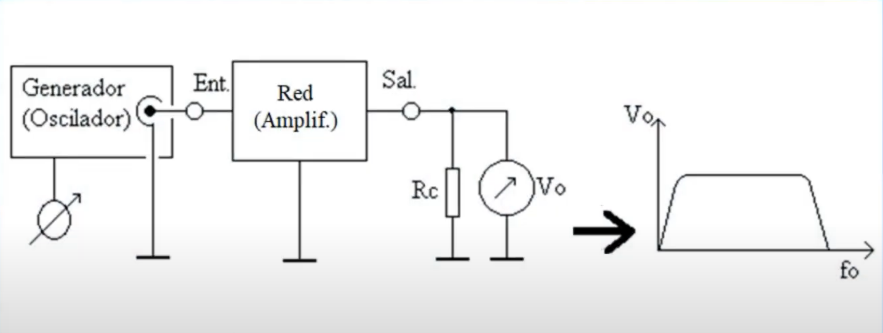
\includegraphics[width=0.6\textwidth]{Imagenes/ActividadPractica/MarcoTeorico/EsquemaGeneradorBarrido.png}}
          \caption{Esquema de barrido en frecuencia.}
          \label{fig:GenBarrido}
      \end{figure}

    Aunque el método propuesto es útil, en la práctica resulta complicado realizar el 
    registro de valores. Como solución al problema planteado, se puede utilizar un generador 
    de barrido el cual posee una salida modulada en frecuencia, ligada a una señal triangular,   
    que también está disponible como salida. Este dispositivo se puede utilizar en conjunto 
    con un osciloscopio, para simular el compartamiento de un analizador de redes, que 
    permite visualizar de forma automática la respuesta en frecuencia. 
    La Figura \ref{fig:GenBarridoRed} muestra un posible esquema de conexión. 

      \begin{figure}[H]
        \centering
          \frame{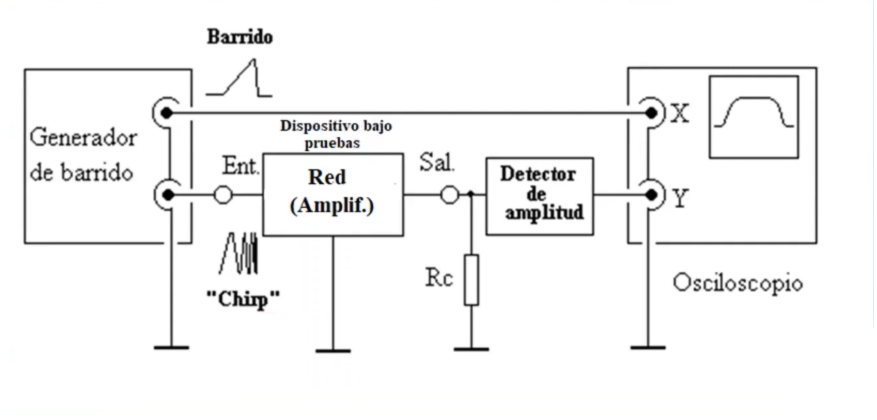
\includegraphics[width=0.6\textwidth]{Imagenes/ActividadPractica/MarcoTeorico/EsquemaGeneradorBarridoYRed.png}}
          \caption{Análisis de red usando un generador de barrido.}
          \label{fig:GenBarridoRed}
      \end{figure}
    
    Con esta segunda alternativa presentada, se logra obtener la respuesta en frecuencia de 
    una red bajo análisis. Sin embargo, no es posible conocer, con exactitud, la frecuencia 
    a la cual pertenece cada medición. Por ésta razón, se hace uso de un generador de marcas.
    La Figura~\ref{fig:GenBarridoYMarca} muestra un generador de barrido y de marcas en 
    conjunto. 
      \begin{figure}[H]
        \centering
          \frame{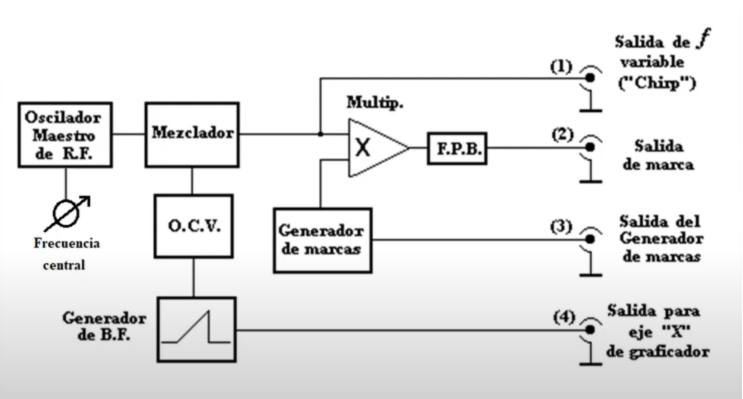
\includegraphics[width=0.6\textwidth]{Imagenes/ActividadPractica/MarcoTeorico/EsquemaGeneradorDeBarridoYMarcas.png}}
          \caption{Esquema de generador de barrido y marcas.}
          \label{fig:GenBarridoYMarca}
      \end{figure}

    La salida de marca proviene de un modulador en conjunto con un filtro pasa bajos 
    (generada con el método del batido cero), que se conoce como \textit{PIP}.
    Dicha señal se suma a la respuesta de la red bajo análisis, y se obtiene la salida 
    del canal vertical. De esta forma, la marca permite determinar la frecuencia. En la 
    Figura~\ref{fig:GenBarridoYMarcaOscilos} se muestra el esquema del análisis de una 
    red con un osciloscopio y un generador de barrido y marcas. 
      \begin{figure}[H]
        \centering
          \frame{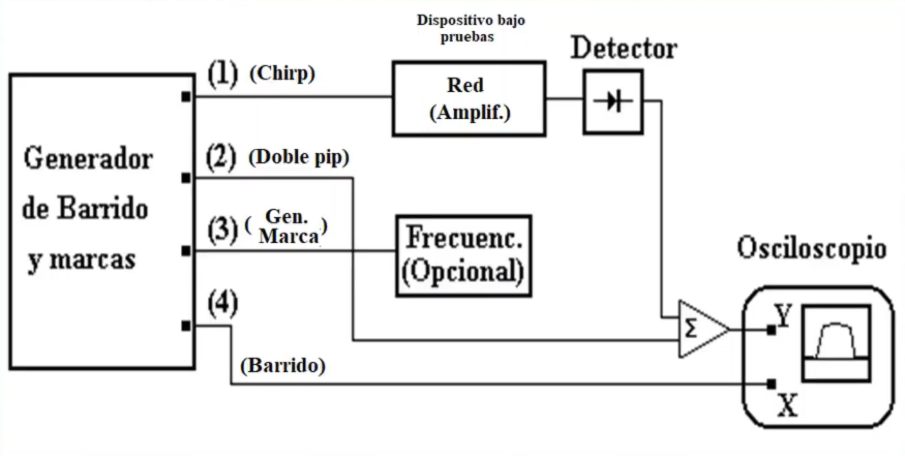
\includegraphics[width=0.6\textwidth]{Imagenes/ActividadPractica/MarcoTeorico/EsquemaGeneradorDeBarridoYMarcasOsciloscopio.png}}
          \caption{Esquema de osciloscopio y generador de barrido y marcas.}
          \label{fig:GenBarridoYMarcaOscilos}
      \end{figure}


    Los ensayos se pueden realizar en un receptor FM, cuyo esquema simplificado se presenta 
    en la Figura \ref{fig:ReceptorSimplificado}.
      \begin{figure}[H]
        \centering
          \frame{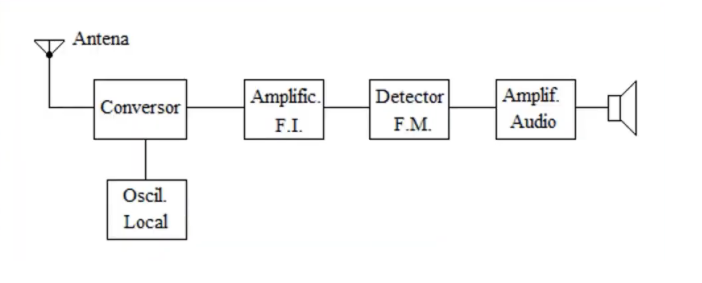
\includegraphics[width=0.6\textwidth]{Imagenes/ActividadPractica/MarcoTeorico/EsquemaSimplificadoReceptorFM.png}}
          \caption{Esquema de Detector FM simplificado.}
          \label{fig:ReceptorSimplificado}
      \end{figure}

    Se considera como etapa amplificadora, al conjunto formado por el conversor 
    y el amplificador, que conforman lo que se denomina \textit{amplificador sintonizado}.

    La salida del amplificador se combina con el detector para dar la señal resultante. 
    Bajo éste análisis, se deduce la salida del receptor de FM, que muestra la 
    Figura \ref{fig:FdeTReceptor}. Dicha salida es de utilidad para realizar los ensayos 
    propuestos en el presente informe.

      \begin{figure}[H]
        \centering
          \frame{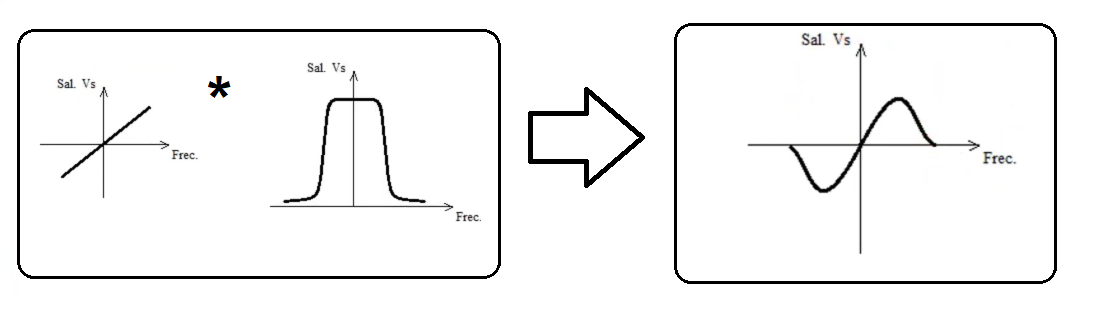
\includegraphics[width=0.6\textwidth]{Imagenes/ActividadPractica/MarcoTeorico/FdeTDetector.png}}
          \caption{Salida del detector.}
          \label{fig:FdeTReceptor}
      \end{figure}


    \pagebreak
  \section{Actividad Práctica}
    Se propone medir la respuesta en frecuencia de un receptor FM mediante un generador de barrido y marcas, junto
    con un osciloscopio analógico. Los instrumentos de los cuales se hace uso son

    \begin{itemize}
      \item Generador de barrido y marcas LSW-250
      \item Osciloscopio analógico Hitachi V-665A
      \item Radio FM
    \end{itemize}

    Para el receptor de FM la etapa detectora será considerada como parte del amplificador de FI (frecuencia intermedia).
    
      \subsection{Calibración del dial del Generador de Barrido}
    A 

      \subsection{Características de detección}

      \subsection{Valores límtes de detección de sintonía}


    \section{Conclusiones}

  Para determinar la frecuencia del oscilador local, se parte sabiendo las frecuencias 
  \(f_{min}\) y \(f_{max}\) del receptor, y
  aplicando el cálculo 
    \begin{equation*}
      FI = \dfrac{f_{max} - f_{min}}{2} + k = 10,7~[Mhz]~,
    \end{equation*}
  donde \(k = 0,7\) para el estándar de FM.
  
  Luego, debido a que el receptor es superheterodino, la 
  frecuencia del oscilador local se determina de la siguiente 
  manera
    
    \begin{equation*}
      f_{osc} = f_{sintonia} +FI .
    \end{equation*}

  
\end{document}
